\documentclass{beamer}
%\usepackage[latin1]{inputenc}
%\usepackage{lmodern}
\usepackage{times}
\usepackage[T1]{fontenc}
\usepackage{graphicx}
\usepackage{bm}
\usepackage{tikz}
\usepackage{verbatim}
\usepackage{amsmath}
\usepackage[small,labelformat=empty]{caption}
\usepackage{url}

\usetheme{Frankfurt}
%\usetheme{Warsaw}
\title[Title of presentation]{Title of presentation\\
{\small possibly subtitle}
}
\author[author name]
{further information <\url{can-include.urls}>}
\institute[Fnord GmbH]{}
\date{23.5.1984 - 42.5.1984}

\begin{document}

\section{uhrenbaustein}
  \begin{frame}{uhrenbaustein - integrate modules}
	  \begin{tikzpicture}
		\end{tikzpicture}
  \end{frame}

  \begin{frame}{uhrenbaustein - supply input signals}
	  \begin{tikzpicture}
		\end{tikzpicture}
  \end{frame}
 
  \begin{frame}{uhrenbaustein - supply output signals}
	  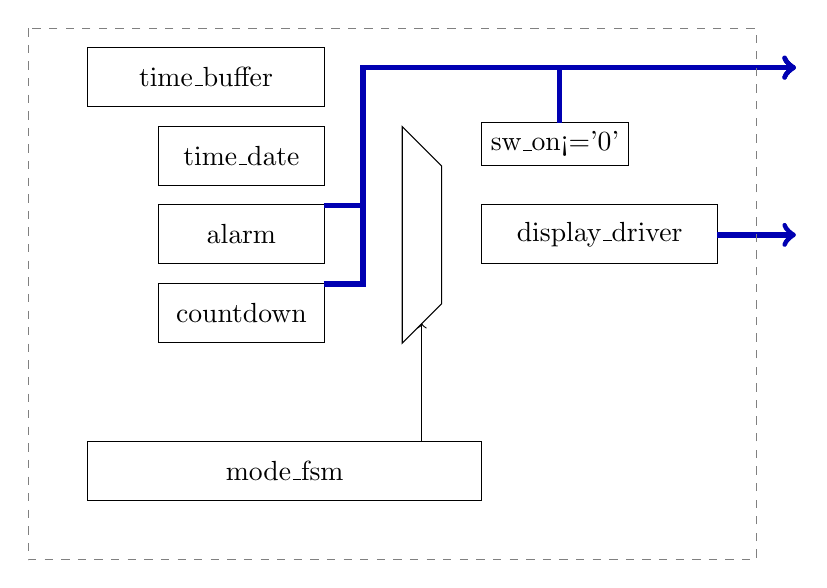
\begin{tikzpicture}
		  % individual modules
		\node[rectangle,draw=black,minimum height=.75cm,minimum width=3cm,above right] at (0,-1) {time\_buffer};
		\node[rectangle,draw=black,minimum height=.75cm,minimum width=2.1cm,above right] at (.9,-2) {time\_date};
		\node[rectangle,draw=black,minimum height=.75cm,minimum width=2.1cm,above right] at (.9,-3) {alarm};
		\node[rectangle,draw=black,minimum height=.75cm,minimum width=2.1cm,above right] at (.9,-4) {countdown};
		\node[rectangle,draw=black,minimum height=.75cm,minimum width=3cm,above right] at (5,-3) {display\_driver};
		\node[rectangle,draw=black,minimum height=.75cm,minimum width=5cm,above right] at (0,-6) {mode\_fsm};

	
    % outputs
		\draw[blue!70!black,line width=2pt,->] (3,-2.25) -- (3.5,-2.25) -- (3.5,-.5) -> (9,-.5);
  	\draw[blue!70!black,line width=2pt,->] (3,-3.25) -- (3.5,-3.25) -- (3.5,-.5) -> (9,-.5);
  	\node[rectangle,draw=black,above right] at (5,-1.75) {sw\_on<='0'};
	  \draw[blue!70!black,line width=2pt,->] (6,-1.2) -- (6,-.5) -> (9,-.5);

		% mux ctl
		\draw[->] (4.25,-5.25) -> (4.25,-3.75);

		% display control lines
	  \draw[blue!70!black,line width=2pt,->] (8,-2.625) -> (9,-2.625);


		% mux
		\draw (4,-1.25) -- (4.5, -1.75) -- (4.5,-3.5) -- (4,-4) -- cycle;

		% top level module
		\draw[dashed,gray] (-.75,0) rectangle (8.5, -6.75);
	\end{tikzpicture}
 \end{frame}
\section{mode\_alarm}
  \begin{frame}{mode\_alarm overview}
    \begin{tikzpicture}
		\node[rectangle,draw=black,minimum height=.75cm,minimum width=1.5cm,above right] at (0,1) {+/-};
	  \node[rectangle,draw=black,minimum height=.75cm,minimum width=1.5cm,above right] at (0,0) {reset};
	  \node[rectangle,draw=black,minimum height=.75cm,minimum width=1.5cm,above right] at (2,-1.25) {Priority};
	  \node[rectangle,draw=black,minimum height=.75cm,minimum width=1.5cm,above right] at (2,-4.5) {NOT};
	  \node[rectangle,draw=black,minimum height=.75cm,minimum width=1.5cm,above right] at (7,-1.5) {Alarm FSM};
	

    % switch alarm active
    \node[rectangle,above right] at (-.5,-4.5) {alarm\_active};
	  \node[rectangle,above right] at (-.5,-5.5) {alarm\_on!='1'};
	  \node[rectangle,above right] at (-.5,-6) {kc\_act\_imp};
		\draw[->] (2,-5.25) -- (2.75,-5.25) -> (2.75,-4.5);
		\draw[->] (1.75,-5.75) -- (3,-5.75) -> (3,-4.5);
	



    \end{tikzpicture}
  \end{frame}

  \begin{frame}{mode\_alarm alarm\_on FSM}
    \begin{tikzpicture}
    \end{tikzpicture}
  \end{frame}
\end{document}

